% Options for packages loaded elsewhere
\PassOptionsToPackage{unicode}{hyperref}
\PassOptionsToPackage{hyphens}{url}
\PassOptionsToPackage{dvipsnames,svgnames,x11names}{xcolor}
%
\documentclass[
  letterpaper,
  DIV=11,
  numbers=noendperiod]{scrartcl}

\usepackage{amsmath,amssymb}
\usepackage{iftex}
\ifPDFTeX
  \usepackage[T1]{fontenc}
  \usepackage[utf8]{inputenc}
  \usepackage{textcomp} % provide euro and other symbols
\else % if luatex or xetex
  \usepackage{unicode-math}
  \defaultfontfeatures{Scale=MatchLowercase}
  \defaultfontfeatures[\rmfamily]{Ligatures=TeX,Scale=1}
\fi
\usepackage{lmodern}
\ifPDFTeX\else  
    % xetex/luatex font selection
\fi
% Use upquote if available, for straight quotes in verbatim environments
\IfFileExists{upquote.sty}{\usepackage{upquote}}{}
\IfFileExists{microtype.sty}{% use microtype if available
  \usepackage[]{microtype}
  \UseMicrotypeSet[protrusion]{basicmath} % disable protrusion for tt fonts
}{}
\makeatletter
\@ifundefined{KOMAClassName}{% if non-KOMA class
  \IfFileExists{parskip.sty}{%
    \usepackage{parskip}
  }{% else
    \setlength{\parindent}{0pt}
    \setlength{\parskip}{6pt plus 2pt minus 1pt}}
}{% if KOMA class
  \KOMAoptions{parskip=half}}
\makeatother
\usepackage{xcolor}
\setlength{\emergencystretch}{3em} % prevent overfull lines
\setcounter{secnumdepth}{5}
% Make \paragraph and \subparagraph free-standing
\ifx\paragraph\undefined\else
  \let\oldparagraph\paragraph
  \renewcommand{\paragraph}[1]{\oldparagraph{#1}\mbox{}}
\fi
\ifx\subparagraph\undefined\else
  \let\oldsubparagraph\subparagraph
  \renewcommand{\subparagraph}[1]{\oldsubparagraph{#1}\mbox{}}
\fi


\providecommand{\tightlist}{%
  \setlength{\itemsep}{0pt}\setlength{\parskip}{0pt}}\usepackage{longtable,booktabs,array}
\usepackage{calc} % for calculating minipage widths
% Correct order of tables after \paragraph or \subparagraph
\usepackage{etoolbox}
\makeatletter
\patchcmd\longtable{\par}{\if@noskipsec\mbox{}\fi\par}{}{}
\makeatother
% Allow footnotes in longtable head/foot
\IfFileExists{footnotehyper.sty}{\usepackage{footnotehyper}}{\usepackage{footnote}}
\makesavenoteenv{longtable}
\usepackage{graphicx}
\makeatletter
\def\maxwidth{\ifdim\Gin@nat@width>\linewidth\linewidth\else\Gin@nat@width\fi}
\def\maxheight{\ifdim\Gin@nat@height>\textheight\textheight\else\Gin@nat@height\fi}
\makeatother
% Scale images if necessary, so that they will not overflow the page
% margins by default, and it is still possible to overwrite the defaults
% using explicit options in \includegraphics[width, height, ...]{}
\setkeys{Gin}{width=\maxwidth,height=\maxheight,keepaspectratio}
% Set default figure placement to htbp
\makeatletter
\def\fps@figure{htbp}
\makeatother
% definitions for citeproc citations
\NewDocumentCommand\citeproctext{}{}
\NewDocumentCommand\citeproc{mm}{%
  \begingroup\def\citeproctext{#2}\cite{#1}\endgroup}
\makeatletter
 % allow citations to break across lines
 \let\@cite@ofmt\@firstofone
 % avoid brackets around text for \cite:
 \def\@biblabel#1{}
 \def\@cite#1#2{{#1\if@tempswa , #2\fi}}
\makeatother
\newlength{\cslhangindent}
\setlength{\cslhangindent}{1.5em}
\newlength{\csllabelwidth}
\setlength{\csllabelwidth}{3em}
\newenvironment{CSLReferences}[2] % #1 hanging-indent, #2 entry-spacing
 {\begin{list}{}{%
  \setlength{\itemindent}{0pt}
  \setlength{\leftmargin}{0pt}
  \setlength{\parsep}{0pt}
  % turn on hanging indent if param 1 is 1
  \ifodd #1
   \setlength{\leftmargin}{\cslhangindent}
   \setlength{\itemindent}{-1\cslhangindent}
  \fi
  % set entry spacing
  \setlength{\itemsep}{#2\baselineskip}}}
 {\end{list}}
\usepackage{calc}
\newcommand{\CSLBlock}[1]{\hfill\break\parbox[t]{\linewidth}{\strut\ignorespaces#1\strut}}
\newcommand{\CSLLeftMargin}[1]{\parbox[t]{\csllabelwidth}{\strut#1\strut}}
\newcommand{\CSLRightInline}[1]{\parbox[t]{\linewidth - \csllabelwidth}{\strut#1\strut}}
\newcommand{\CSLIndent}[1]{\hspace{\cslhangindent}#1}

\usepackage{booktabs}
\usepackage{longtable}
\usepackage{array}
\usepackage{multirow}
\usepackage{wrapfig}
\usepackage{float}
\usepackage{colortbl}
\usepackage{pdflscape}
\usepackage{tabu}
\usepackage{threeparttable}
\usepackage{threeparttablex}
\usepackage[normalem]{ulem}
\usepackage{makecell}
\usepackage{xcolor}
\KOMAoption{captions}{tableheading}
\makeatletter
\@ifpackageloaded{caption}{}{\usepackage{caption}}
\AtBeginDocument{%
\ifdefined\contentsname
  \renewcommand*\contentsname{Table of contents}
\else
  \newcommand\contentsname{Table of contents}
\fi
\ifdefined\listfigurename
  \renewcommand*\listfigurename{List of Figures}
\else
  \newcommand\listfigurename{List of Figures}
\fi
\ifdefined\listtablename
  \renewcommand*\listtablename{List of Tables}
\else
  \newcommand\listtablename{List of Tables}
\fi
\ifdefined\figurename
  \renewcommand*\figurename{Figure}
\else
  \newcommand\figurename{Figure}
\fi
\ifdefined\tablename
  \renewcommand*\tablename{Table}
\else
  \newcommand\tablename{Table}
\fi
}
\@ifpackageloaded{float}{}{\usepackage{float}}
\floatstyle{ruled}
\@ifundefined{c@chapter}{\newfloat{codelisting}{h}{lop}}{\newfloat{codelisting}{h}{lop}[chapter]}
\floatname{codelisting}{Listing}
\newcommand*\listoflistings{\listof{codelisting}{List of Listings}}
\makeatother
\makeatletter
\makeatother
\makeatletter
\@ifpackageloaded{caption}{}{\usepackage{caption}}
\@ifpackageloaded{subcaption}{}{\usepackage{subcaption}}
\makeatother
\ifLuaTeX
  \usepackage{selnolig}  % disable illegal ligatures
\fi
\usepackage{bookmark}

\IfFileExists{xurl.sty}{\usepackage{xurl}}{} % add URL line breaks if available
\urlstyle{same} % disable monospaced font for URLs
\hypersetup{
  pdftitle={Exploring TTC Delays},
  pdfauthor={Luca Carnegie},
  colorlinks=true,
  linkcolor={blue},
  filecolor={Maroon},
  citecolor={Blue},
  urlcolor={Blue},
  pdfcreator={LaTeX via pandoc}}

\title{Exploring TTC Delays\thanks{Code and data are available at:
https://github.com/lcarnegie/OpenDataToronto. Thank you to Nescafé
coffee, Rajan Maghera, Hannah Yu, and Sehar Bajwa for your love and
support - could not have done it without you. No thanks go to Rohan in
particular for not pointing out all the R he wanted us to learn that was
in his textbook\ldots{} sigh. I will try the appendix cocktails someday,
though. :)}}
\usepackage{etoolbox}
\makeatletter
\providecommand{\subtitle}[1]{% add subtitle to \maketitle
  \apptocmd{\@title}{\par {\large #1 \par}}{}{}
}
\makeatother
\subtitle{A Multimodal Analysis}
\author{Luca Carnegie}
\date{January 25, 2024}

\begin{document}
\maketitle
\begin{abstract}
First sentence. Second sentence. Third sentence. Fourth sentence.
\end{abstract}

\section{Introduction}\label{introduction}

A key area of improvement in Canadian sustainability is in increasing
the use of public transportation in big cities like Toronto. This makes
sense, since cars account for about 80\% of transportation emissions
(Dia et al. 2019). A major drawback preventing the widespread use of
public transportation is the existence of delays within transit systems.
These delays push citizens toward using less sustainable alternatives
like private cars, leading to congestion on highways and consequent
increased emissions. The lack of timely transit services have a
demonstrated impact on traffic. One study by Anderson et al.~estimated a
whopping 47 percent increase in highway delay when transit service
ceased completely in a big city such as Los Angeles (Anderson 2014).
Learning from this example, it is imperative that policy makers
understand and fix these delays to improve sustainability in Toronto.

The Toronto Transit Commission (TTC) has been Toronto's transit system
since 1921, serving the city population with a variety of transportation
methods, particularly subways, streetcars, and buses. The openly
available data surrounding the delays of these various modes of
transport offers the opportunity to investigate the root causes of these
delays and prompt discussion as how to rectify them. Understanding the
common causes of a delay, when a delay is typically caused and where it
was caused gives the TTC more insight into how to deliver their services
to the public more efficiently and effectively, setting an improved
example of what an effective transit agency looks like.

This paper aims to find patterns of public transit delay time across
various genres of transportation. First, the data source and analysis
employed are covered in Section Two. Section Three then critically
examines the data, delving deeper to arrive at various conclusions, as
well as discussing implications and proposing new areas of exploration
for this data.

\section{Data}\label{sec-data}

To investigate transit delays in Toronto, data on bus (Commission
2024a), subway (Commission 2024c), and streetcar (Commission 2024b)
delay incidents for the year 2023 was downloaded using the
OpenDataToronto R package (Gelfand 2022). Then, the data was cleaned
using R (R Core Team 2022), tidyverse (Wickham et al. 2019) and it's
associated packages. After combining the datasets together, variables
common between datasets and relevant to the analysis were selected,
leading to a dataset with 93,569 observations. In the case of this
analysis, the variables included were date (year, month, day), day of
the week, Location of Delay Incident, Cause of Delay, the time delay (in
minutes), Vehicle (bus, subway, streetcar), as well as the route/line
(simplified to `line') the vehicle was on when the incident happened.

\begin{table}

\caption{\label{tbl-cleaned\_data}Sample of Cleaned Delay Data}

\centering{

}

\end{table}%

\begin{table}
\caption{Sample of Cleaned Delay Data}\tabularnewline

\centering
\resizebox{\linewidth}{!}{
\begin{tabular}{l|l|l|l|r|l|l|r}
\hline
Date & Time & Day & Vehicle & Route/Line & Location & Reason & Delay (Minutes)\\
\hline
\cellcolor{gray!6}{2023-01-01} & \cellcolor{gray!6}{02:30:00} & \cellcolor{gray!6}{Sunday} & \cellcolor{gray!6}{Bus} & \cellcolor{gray!6}{91} & \cellcolor{gray!6}{WOODBINE AND MORTIMER} & \cellcolor{gray!6}{Diversion} & \cellcolor{gray!6}{81}\\
\hline
2023-01-01 & 02:34:00 & Sunday & Bus & 69 & WARDEN STATION & Security & 22\\
\hline
\cellcolor{gray!6}{2023-01-01} & \cellcolor{gray!6}{03:06:00} & \cellcolor{gray!6}{Sunday} & \cellcolor{gray!6}{Bus} & \cellcolor{gray!6}{35} & \cellcolor{gray!6}{JANE STATION} & \cellcolor{gray!6}{Cleaning} & \cellcolor{gray!6}{30}\\
\hline
2023-01-01 & 03:14:00 & Sunday & Bus & 900 & KIPLING STATION & Security & 17\\
\hline
\cellcolor{gray!6}{2023-01-01} & \cellcolor{gray!6}{03:43:00} & \cellcolor{gray!6}{Sunday} & \cellcolor{gray!6}{Bus} & \cellcolor{gray!6}{85} & \cellcolor{gray!6}{MEADOWALE LOOP} & \cellcolor{gray!6}{Security} & \cellcolor{gray!6}{1}\\
\hline
\end{tabular}}
\end{table}

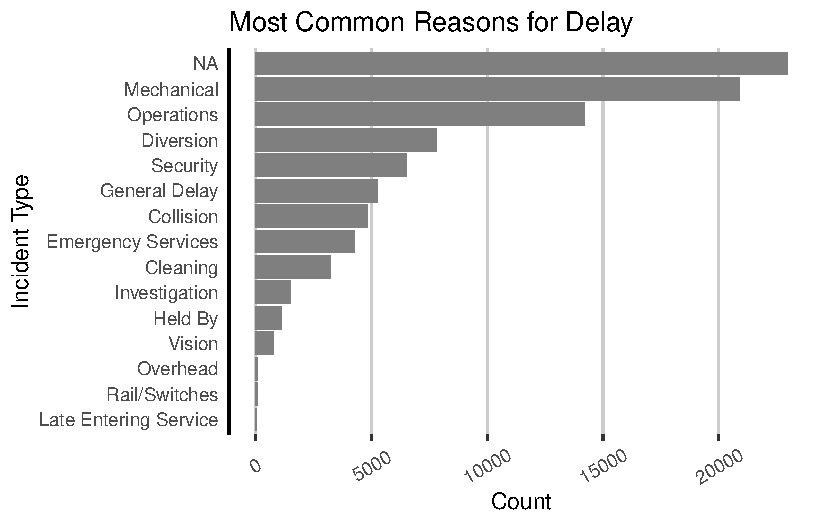
\includegraphics{paper_files/figure-pdf/common-reasons-delay-1.pdf}

\begin{verbatim}
Warning: Unknown or uninitialised column: `month`.
\end{verbatim}

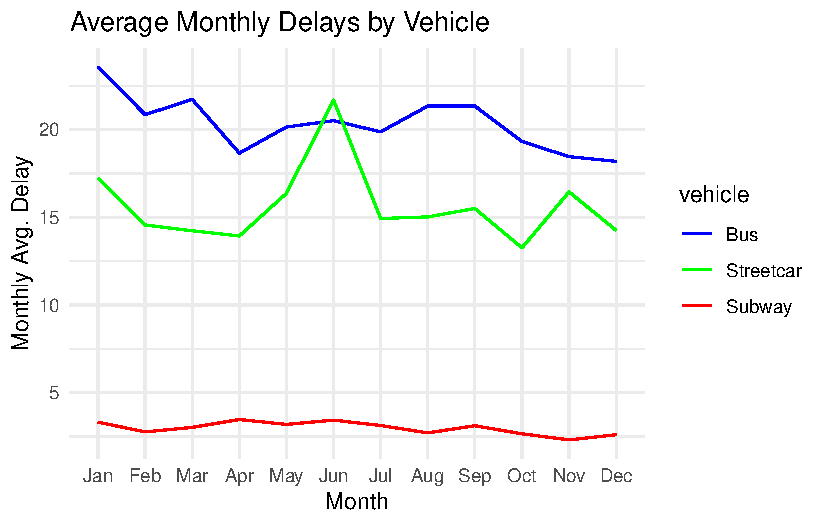
\includegraphics{paper_files/figure-pdf/monthly-delay-times-1.pdf}

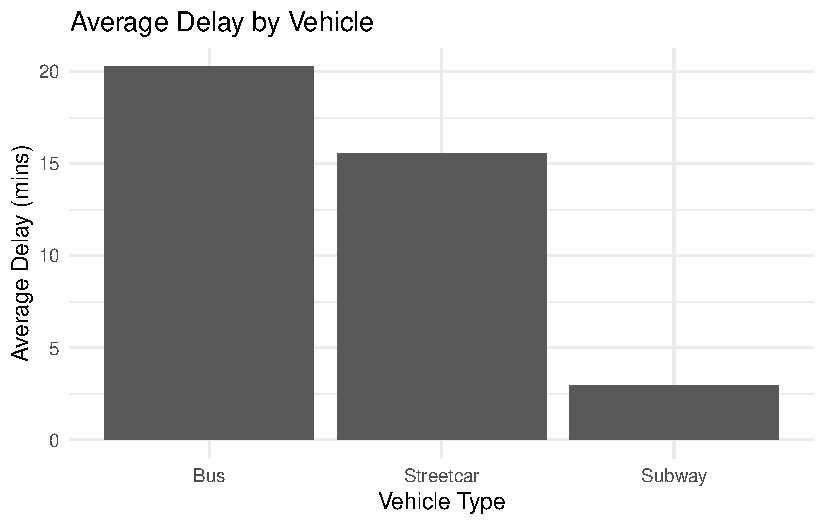
\includegraphics{paper_files/figure-pdf/mode-longest-delays-1.pdf}

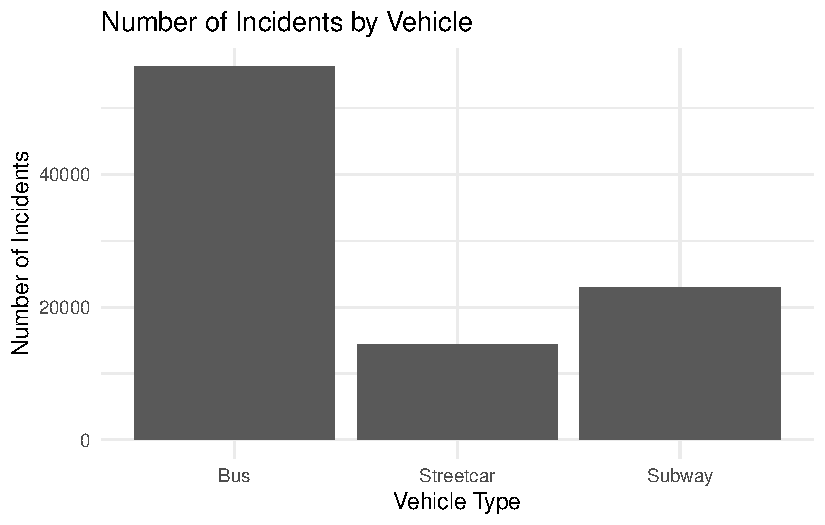
\includegraphics{paper_files/figure-pdf/most-incidents-vehicle-1.pdf}

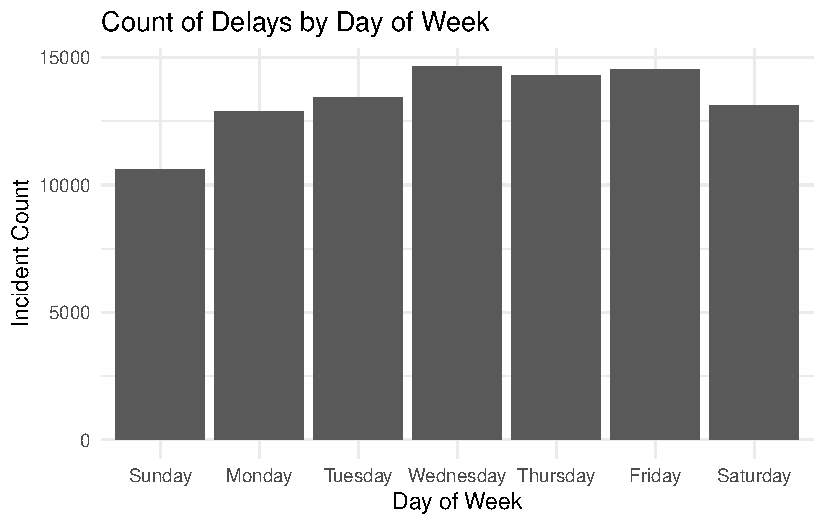
\includegraphics{paper_files/figure-pdf/transport-delay-time-1.pdf}

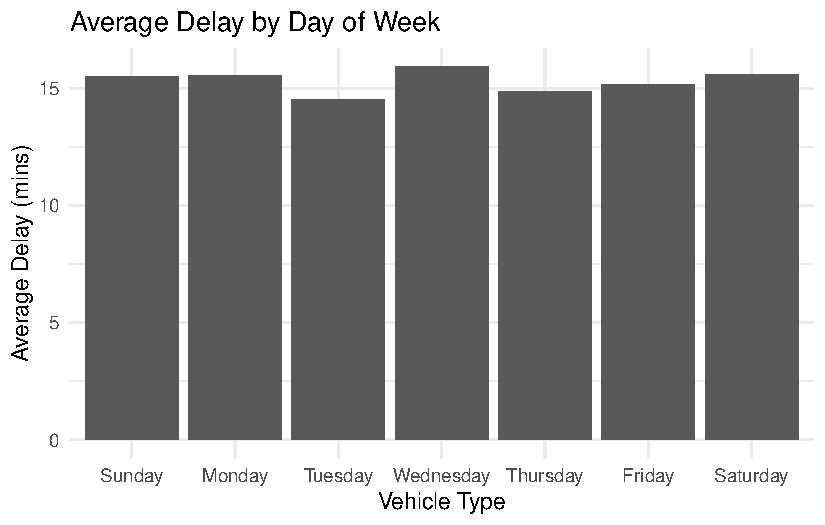
\includegraphics{paper_files/figure-pdf/transport-delay-number-1.pdf}

\section{Discussion}\label{sec-discussion}

\section*{References}\label{references}
\addcontentsline{toc}{section}{References}

\phantomsection\label{refs}
\begin{CSLReferences}{1}{0}
\bibitem[\citeproctext]{ref-anderson}
Anderson, Michael L. 2014. {``Subways, Strikes, and Slowdowns: The
Impacts of Public Transit on Traffic Congestion.''} \emph{American
Economic Review} 104 (9): 2763--96.
\url{https://doi.org/10.1257/aer.104.9.2763}.

\bibitem[\citeproctext]{ref-busdata}
Commission, Toronto Transit. 2024a. {``TTC Bus Delay Data.''}
\url{https://open.toronto.ca/dataset/ttc-bus-delay-data/}.

\bibitem[\citeproctext]{ref-streetcardata}
---------. 2024b. {``TTC Streetcar Delay Data.''}
\url{https://open.toronto.ca/dataset/ttc-streetcar-delay-data/}.

\bibitem[\citeproctext]{ref-subwaydata}
---------. 2024c. {``TTC Subway Delay Data.''}
\url{https://open.toronto.ca/dataset/ttc-subway-delay-data/}.

\bibitem[\citeproctext]{ref-diaetal}
Dia, Hussein, Michael Taylor, John Stone, Sekhar Somenahalli, and
Stephen Cook. 2019. {``Low Carbon Urban Mobility.''} In, 259--85.
\url{https://doi.org/10.1007/978-981-13-7940-6_14}.

\bibitem[\citeproctext]{ref-janitor}
Firke, Sam. 2023. \emph{Janitor: Simple Tools for Examining and Cleaning
Dirty Data}. \url{https://CRAN.R-project.org/package=janitor}.

\bibitem[\citeproctext]{ref-odt}
Gelfand, Sharla. 2022. \emph{Opendatatoronto: Access the City of Toronto
Open Data Portal}.
\url{https://CRAN.R-project.org/package=opendatatoronto}.

\bibitem[\citeproctext]{ref-lubridate}
Grolemund, Garrett, and Hadley Wickham. 2011. {``Dates and Times Made
Easy with {lubridate}.''} \emph{Journal of Statistical Software} 40 (3):
1--25. \url{https://www.jstatsoft.org/v40/i03/}.

\bibitem[\citeproctext]{ref-MartinWittmanLi}
Martin, Layla, Michael Wittmann, and Xinyu Li. 2021. {``The Influence of
Public Transport Delays on Mobility on Demand Services.''}
\emph{Electronics} 10 (4).
\url{https://www.mdpi.com/2079-9292/10/4/379}.

\bibitem[\citeproctext]{ref-citeR}
R Core Team. 2022. \emph{R: A Language and Environment for Statistical
Computing}. Vienna, Austria: R Foundation for Statistical Computing.
\url{https://www.R-project.org/}.

\bibitem[\citeproctext]{ref-testthat}
Wickham, Hadley. 2011. {``Testthat: Get Started with Testing.''}
\emph{The R Journal} 3: 5--10.
\url{https://journal.r-project.org/archive/2011-1/RJournal_2011-1_Wickham.pdf}.

\bibitem[\citeproctext]{ref-ggplot}
---------. 2016. \emph{Ggplot2: Elegant Graphics for Data Analysis}.
Springer-Verlag New York. \url{https://ggplot2.tidyverse.org}.

\bibitem[\citeproctext]{ref-tidyverse}
Wickham, Hadley, Mara Averick, Jennifer Bryan, Winston Chang, Lucy
D'Agostino McGowan, Romain François, Garrett Grolemund, et al. 2019.
{``Welcome to the {tidyverse}.''} \emph{Journal of Open Source Software}
4 (43): 1686. \url{https://doi.org/10.21105/joss.01686}.

\bibitem[\citeproctext]{ref-dplyr}
Wickham, Hadley, Romain François, Lionel Henry, Kirill Müller, and Davis
Vaughan. 2023. \emph{Dplyr: A Grammar of Data Manipulation}.
\url{https://CRAN.R-project.org/package=dplyr}.

\end{CSLReferences}



\end{document}
